\section{Growth of non-axisymmetric modes without the influence of the
  planet}
In this section, the planet is introduced at $t=20P_0$ and 
its potential switched on over $10P_0$. At $t=30P_0$ we switch off the
planet potential and azimuthally average the surface density, energy
and velocity fields. At this point the planet has carved a partial
gap. We then perturb the surface density for $r>r_p$ and continue to 
evolve the disc. We impose  sinusoidal perturbations with 
azimuthal wavenumbers $m\in[1,10]$. {\bf what are PERTMIN and PERTMAX values?}  
This procedure allows us to analyse the growth of 
non-axisymmetric modes associated with the gap, but without
complications from non-axisymmetry arising directly from disc-planet
interaction.

Note that these `planet-off' simulations are not linear stability
calculations because since the cooling term in our energy equation
restores the initial temperature profile corresponding to $H/r=0.05$,
rather than the heated gap edge. Linear stability calculations and
adiabatic cases will be further discussed in
section~\ref{adiabatic_section}.  


Simulations here employ a resolution of $(N_r,N_{\phi})=(1024,2048)$
and we consider 
%for a time up to $200P_0$ allowing high resolution and detection of high
%$m$ structures.
cases of $\tilde{\beta}=0.1,1,10$ corresponding to fast, moderate,
and slowly cooled discs.  

\subsection{Gap structure}
%Since stability of the gap is of interest 
We first examine the gap structure formed by planet-disc
interaction as a function of the cooling time. The azimuthally-averaged 
gap profiles are shown in Fig. \ref{intial1D} for varying
$\tilde\beta$. Gaps formed with lower $\tilde\beta$ (faster cooling)
are deeper with steeper gradients at the gap edges. Faster cooling rates also 
increase and decrease the surface density maxima and 
minima increase, respectively. However, a clean gap does not form
in this short time period. 

%For all cases the gap width is $\approx 5r_{hill}$
%which is set by torque balances in the disk \citep{crida06}. 

Larger $\tilde\beta$ values result in higher disc aspect ratios $h=H/r$,
i.e. higher temperatures. Heating mostly occur at the gap edges
due to planet-induced spiral shocks. Decreasing the cooling time
implies that this heat is retained in the disc. In the inviscid limit the gap
opening condition is $r_h\gtrsim H$ or $q\gtrsim 3h^3$
\citep{crida06}. 
% which is a value directly correlated to temperature in our model. 
%For a planet to carve a gap in the surrounding material it has been
%shown that $q>H^3$ is needed \citep{crida06}. 
This indicates that for hotter discs (higher
$h$), it becomes more difficult for a planet of fixed $q$ to open a
gap. This explains the shallower gaps in surface density when
$\tilde{\beta}$ is increased. 

%This is seen in our simulations as changes in $\tilde{\beta}$
%result in changes of $h$ by less than $20\%$ yet gap depth almost
%doubles. 

The important consequence of a heated gap edge is that the
generalized vortensity profiles become smoother with increasing
cooling times, with the extrema becoming less pronounced. Previous locally
isothermal disc-planet simulations show the RWI associated with PV
minima \citep{li05,lin10}. We can therefore expect the RWI to be associated with
minima in the generalized vortensity (corresponding to local surface
density maxima) in the non-isothermal case. Because the extrema are
less sharp, the RWI is expected to be weaker and the gap to be more
stable with longer cooling times.  

%Charactereristicly
%for such disk-planet Rossby vortices the generalized vortensity
%minima correspond to density maxima in the disk. 
%Since generalized vortensity extrema are also
% correspondingly less pronounced and density gradients become smaller
% we expect that the stability of gaps to increase with larger
% $\tilde{\beta}$. 

\begin{figure}
  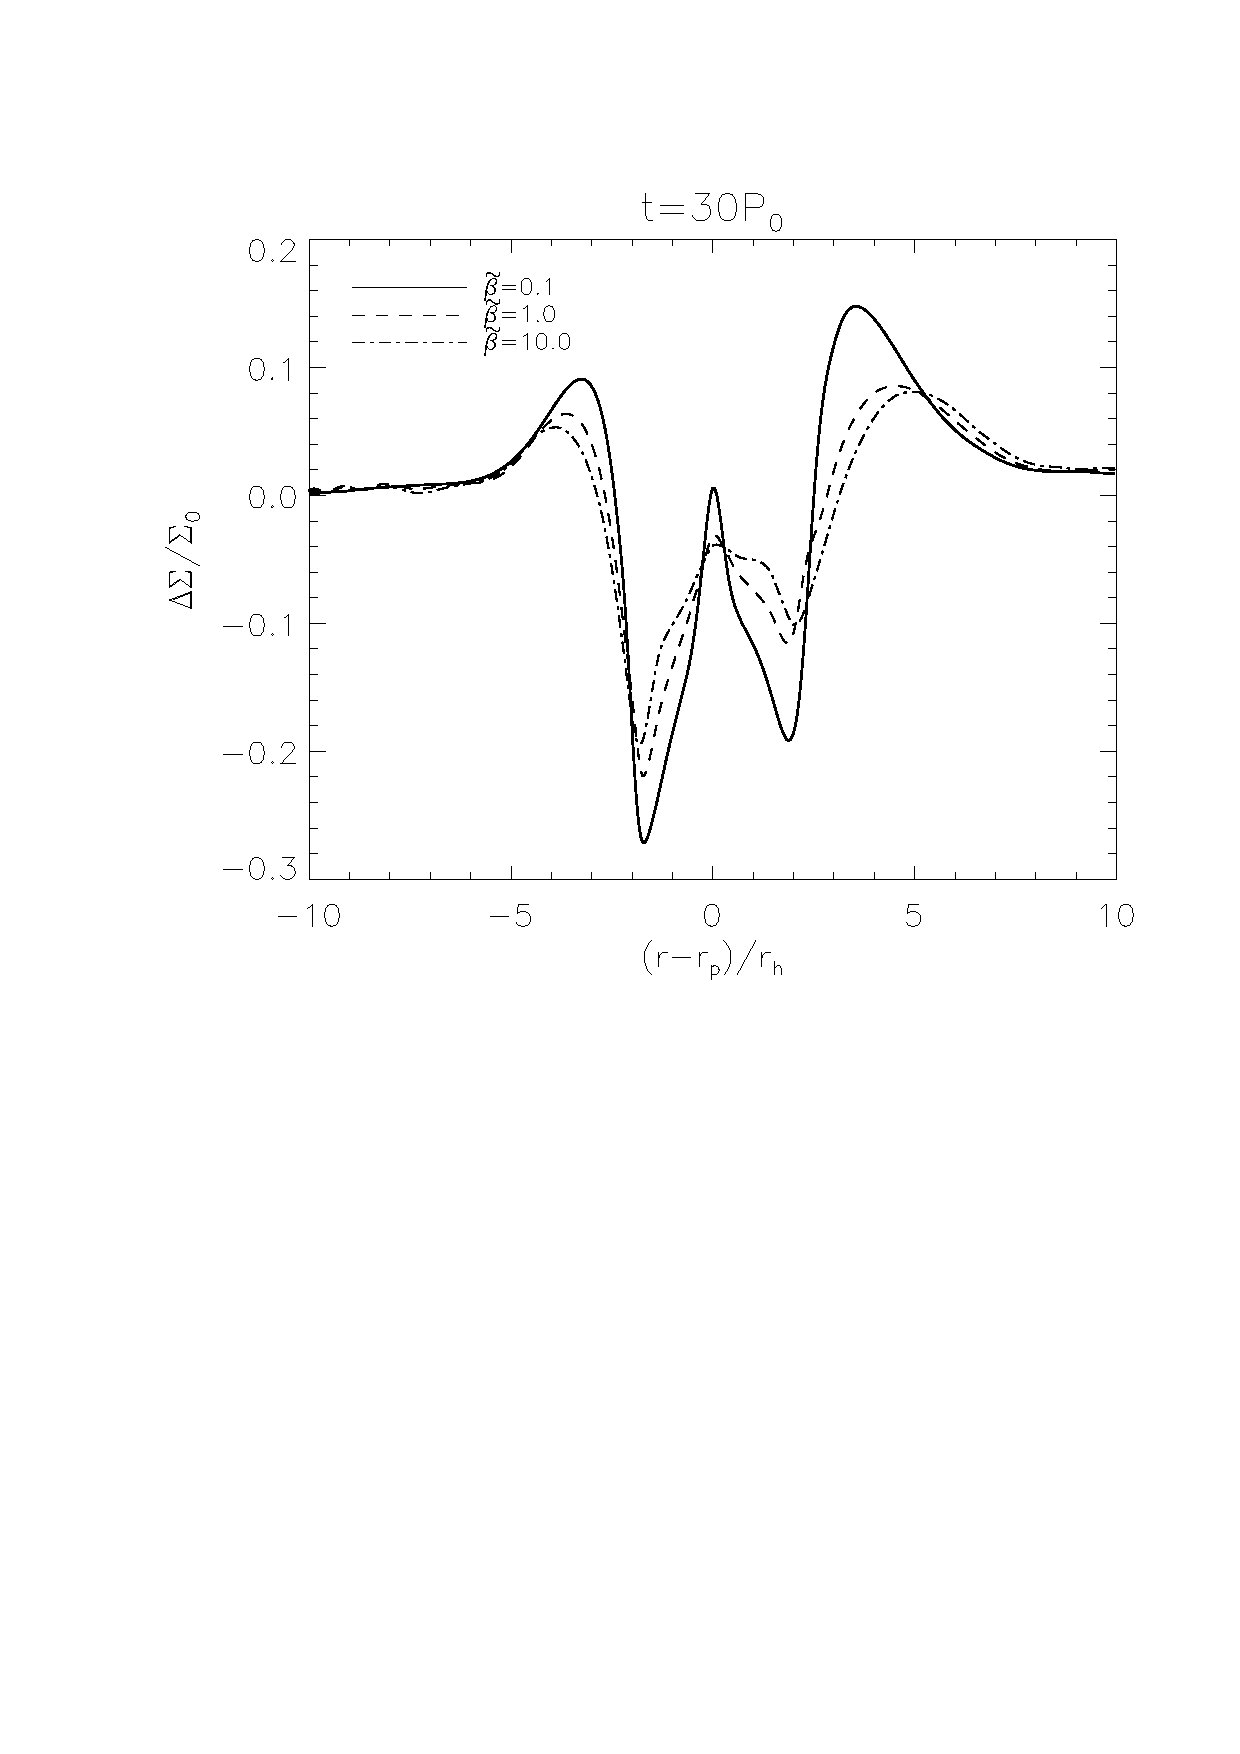
\includegraphics[width=\linewidth,clip=true,trim=0.5cm
    2cm 0cm 0cm]{figures/compare_sigma}
  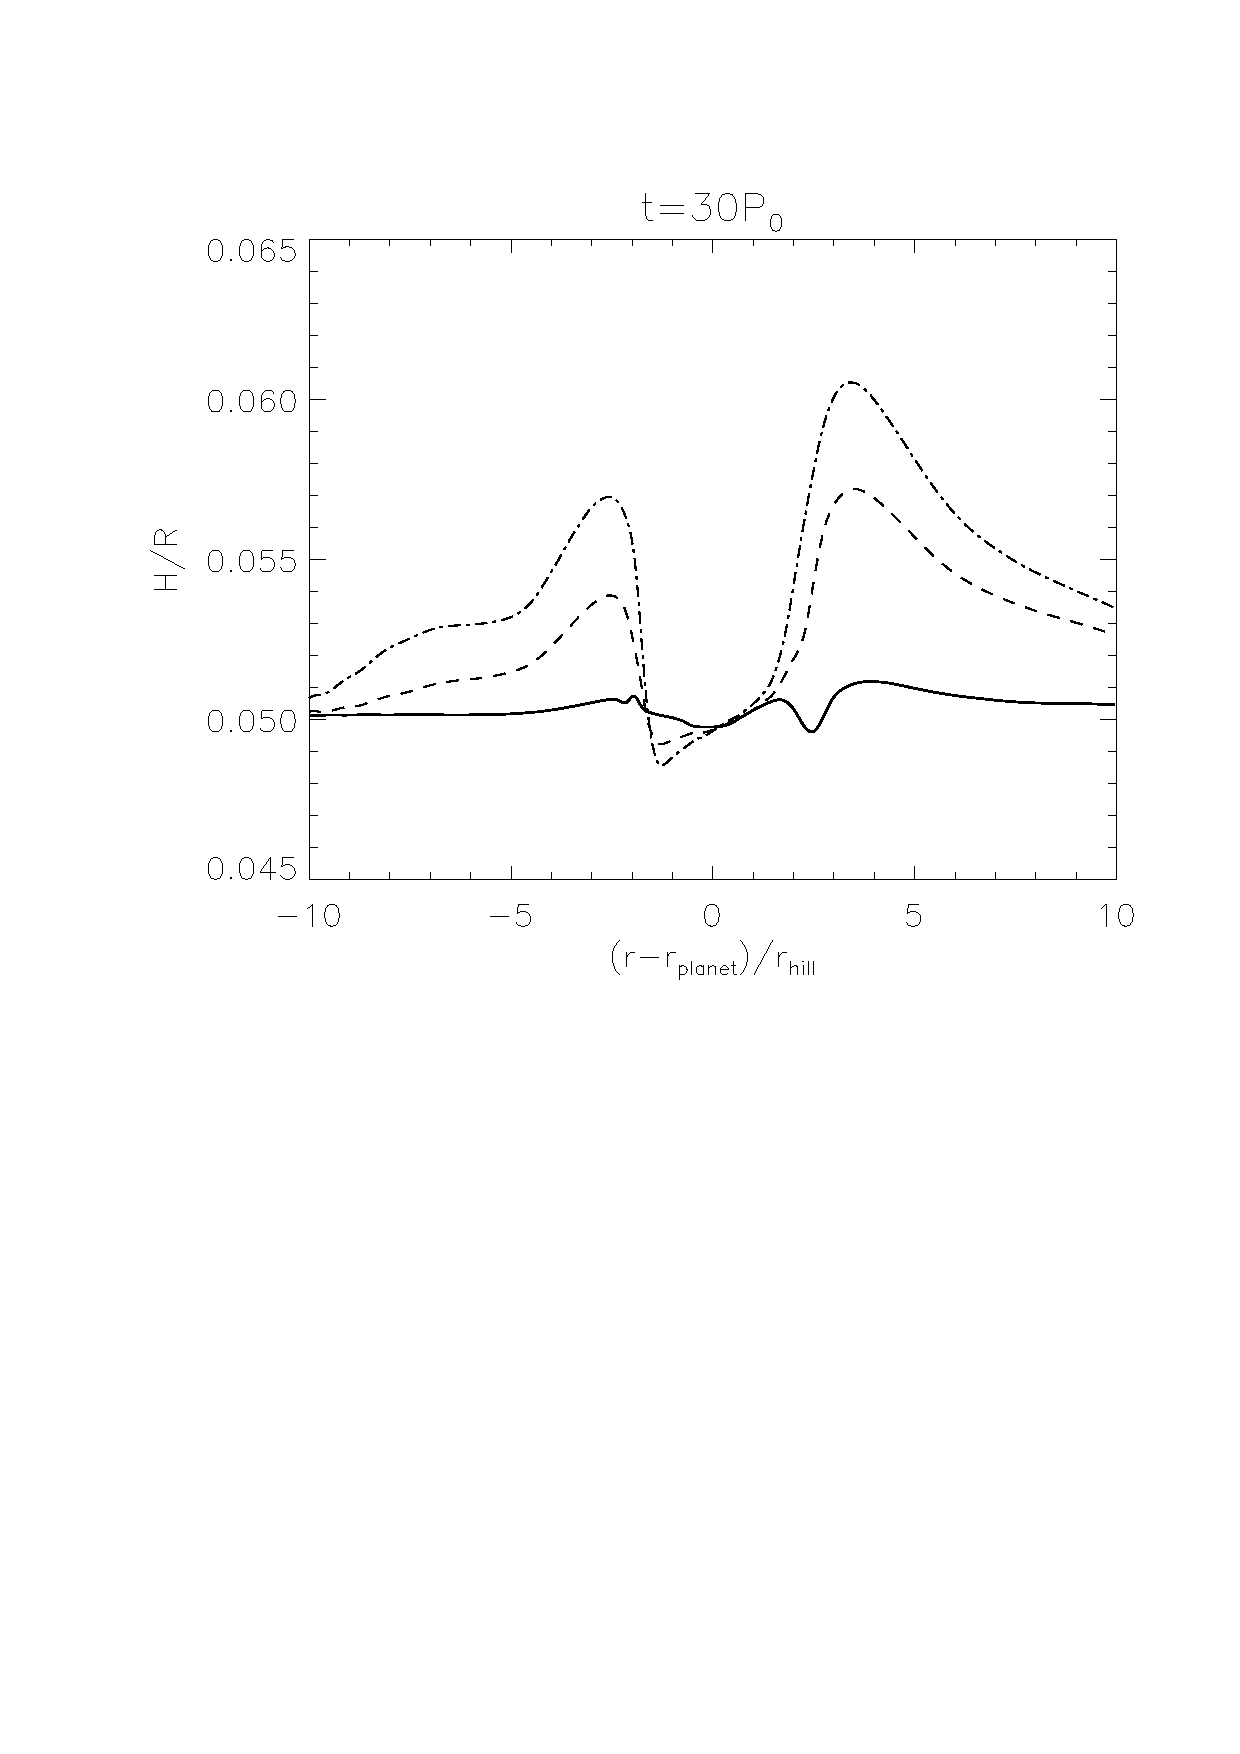
\includegraphics[width=\linewidth,clip=true,trim=0.5cm
    2cm 0cm 1cm]{figures/compare_aspectratio}
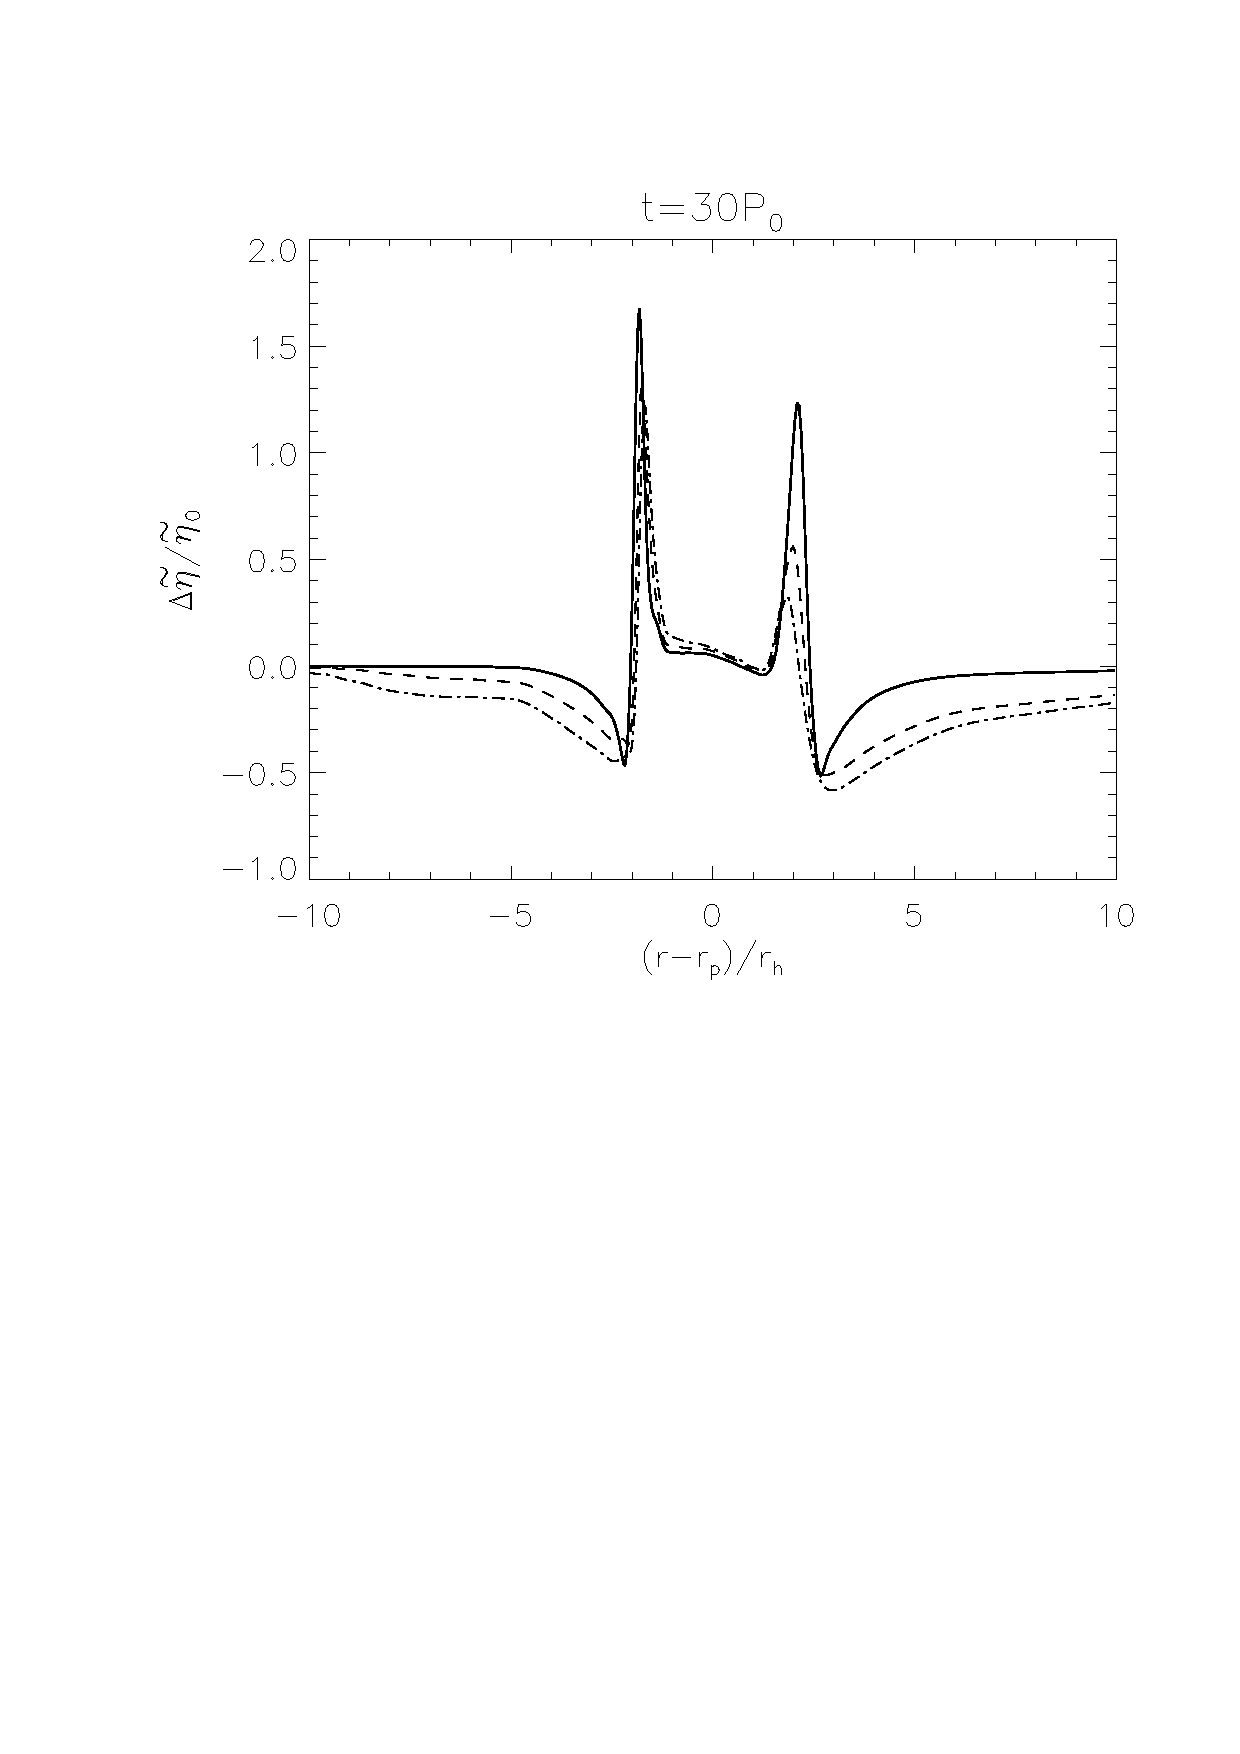
\includegraphics[width=\linewidth,clip=true,trim=0.5cm
    0.5cm 0cm 1cm]{figures/compare_gvortensity}
  \caption{Gap profiles at $t=30P_0$ for the intial partial gap opened
    before instability emerges for fast (solid), moderate
    (dashed), and slow cooling (dashed-dot). The relative surface density
    pertibation (top), disc aspectratio (middle) and generalized
    vortensity pertibation (bottom) are shown. \label{intial1D}}  
\end{figure}


%\begin{tabularx}{0.4\textwidth}{l*{10}{R}} \toprule
%  \multicolumn{11}{c}{$\tilde{\beta}=0.1$} \\ \midrule
%  m                    & 1 & 2 & 3 & 4 & 5 & 6 & 7 & 8 & 9 & 10  \\ 
 % $\gamma10^2/\Omega(r_o)$ & 6.56 & 6.82 & 6.73 & 5.78 & 6.00 & 6.38 & 5.97 & 5.62 & 4.61 & 3.36   \\ \bottomrule
%\end{tabularx}

%\begin{tabularx}{0.4\textwidth}{l*{5}{R}} \toprule
%  \multicolumn{6}{c}{$\tilde{\beta}=1.0$} \\ \midrule
%  m                    & 1 & 2 & 3 & 4 & 5  \\ 
%  $\gamma10^2/\Omega(r_o)$ & 1.27 & 1.28 & 1.35 & 1.01 & 0.61   \\ \bottomrule
%\end{tabularx}

\begin{table}
  \centering
  \caption{Dominant mode and growth rates for
    $\tilde{\beta}=0.1,1.0,10.0$ (fast, moderate, and slow cooling)
    values during `planet-off' simulations \label{modetable}} 
  \hfill
  \begin{minipage}{0.3\linewidth}
    \begin{tabularx}{\textwidth}{l R} 
      \multicolumn{2}{c}{$\tilde{\beta}=0.1$} \\ 
      \toprule
      $m$ & $10^2\gamma/\Omega(r_p)$ \\
      \midrule
      6 & 7.3 \\
      7 & 7.8 \\
      8 & 7.9 \\
      9 & 7.9 \\
      10 & 6.8 \\ 
      \bottomrule
    \end{tabularx}
  \end{minipage}
  \hfill
  \begin{minipage}{0.3\linewidth}
    \begin{tabularx}{\textwidth}{l R} 
      \multicolumn{2}{c}{$\tilde{\beta}=1.0$} \\ 
      \toprule
      $m$ & $10^2\gamma/\Omega(r_p)$ \\
      \midrule
      3 & 2.0 \\
      4 & 2.2 \\
      5 & 2.3 \\
      6 & 1.6 \\
      7 & 1.1 \\ 
      \bottomrule
    \end{tabularx}
  \end{minipage}
  \hfill
  \begin{minipage}{0.3\linewidth}
    \begin{tabularx}{\textwidth}{l R} 
      \multicolumn{2}{c}{$\tilde{\beta}=10.0$} \\ 
      \toprule
      $m$ & $10^2\gamma/\Omega(r_p)$ \\
      \midrule
      1 & 1.1 \\
      2 & 1.6 \\
      3 & 1.7 \\
      4 & 1.2 \\
      5 & 0.1 \\ 
      \bottomrule
    \end{tabularx}
  \end{minipage}
  \hfill
\end{table}

{\bf
\subsection{Axisymmetric stability}
Check that the gap profiles are stable against axisymmetric
stability. Can use analytical criteria given in section 3.1 of Li et
al (2000, ApJ, 533, 1023). No plot needed, just statements. 
}

\subsection{Non-axisymmetric instability}\label{linear}
%{\bf present `planet-off' simulations. one `fourier mode v.s. time'
%  plot to show growth of linear instability. do an adiabatic case (or
%  extremely long cooling time) to see the effect of heated gap edge
%  (i.e. temp doesn't go back to t=0 value too quickly)
%  compare growth rate and dominant
%  m as function of beta (table). 2D figs to contrast (also used to
%  show it's the minimum in generalized pv that goes unstable.    
%  result: increasing cooling time makes the gap
%  more stable, and favors lower m. note: the `basic state' should be
%  the system at t=30 after azimuthal average. linear results should
%  have small perturbations. 
%}

%After the azimuthal averaging, the small pertibation excites rapidly
%growing instabilities by the RWI. 

In all cases we observe growth of non-axisymmetric structures after the
planet potential is switched off and the system subject to random
perturbations. An example is shown in Fig. \ref{linearmodes} for 
$\tilde{\beta}=10$. We charcterize these
modes with an azimuthal wavenumber $m$ and growth rate $\gamma(m)$ as defined by
Eq.~\ref{fouriertransform}---\ref{growth}. Table \ref{modetable}
lists the growth rates for the three cooling
times, measured during linear growth. 


\begin{figure}
  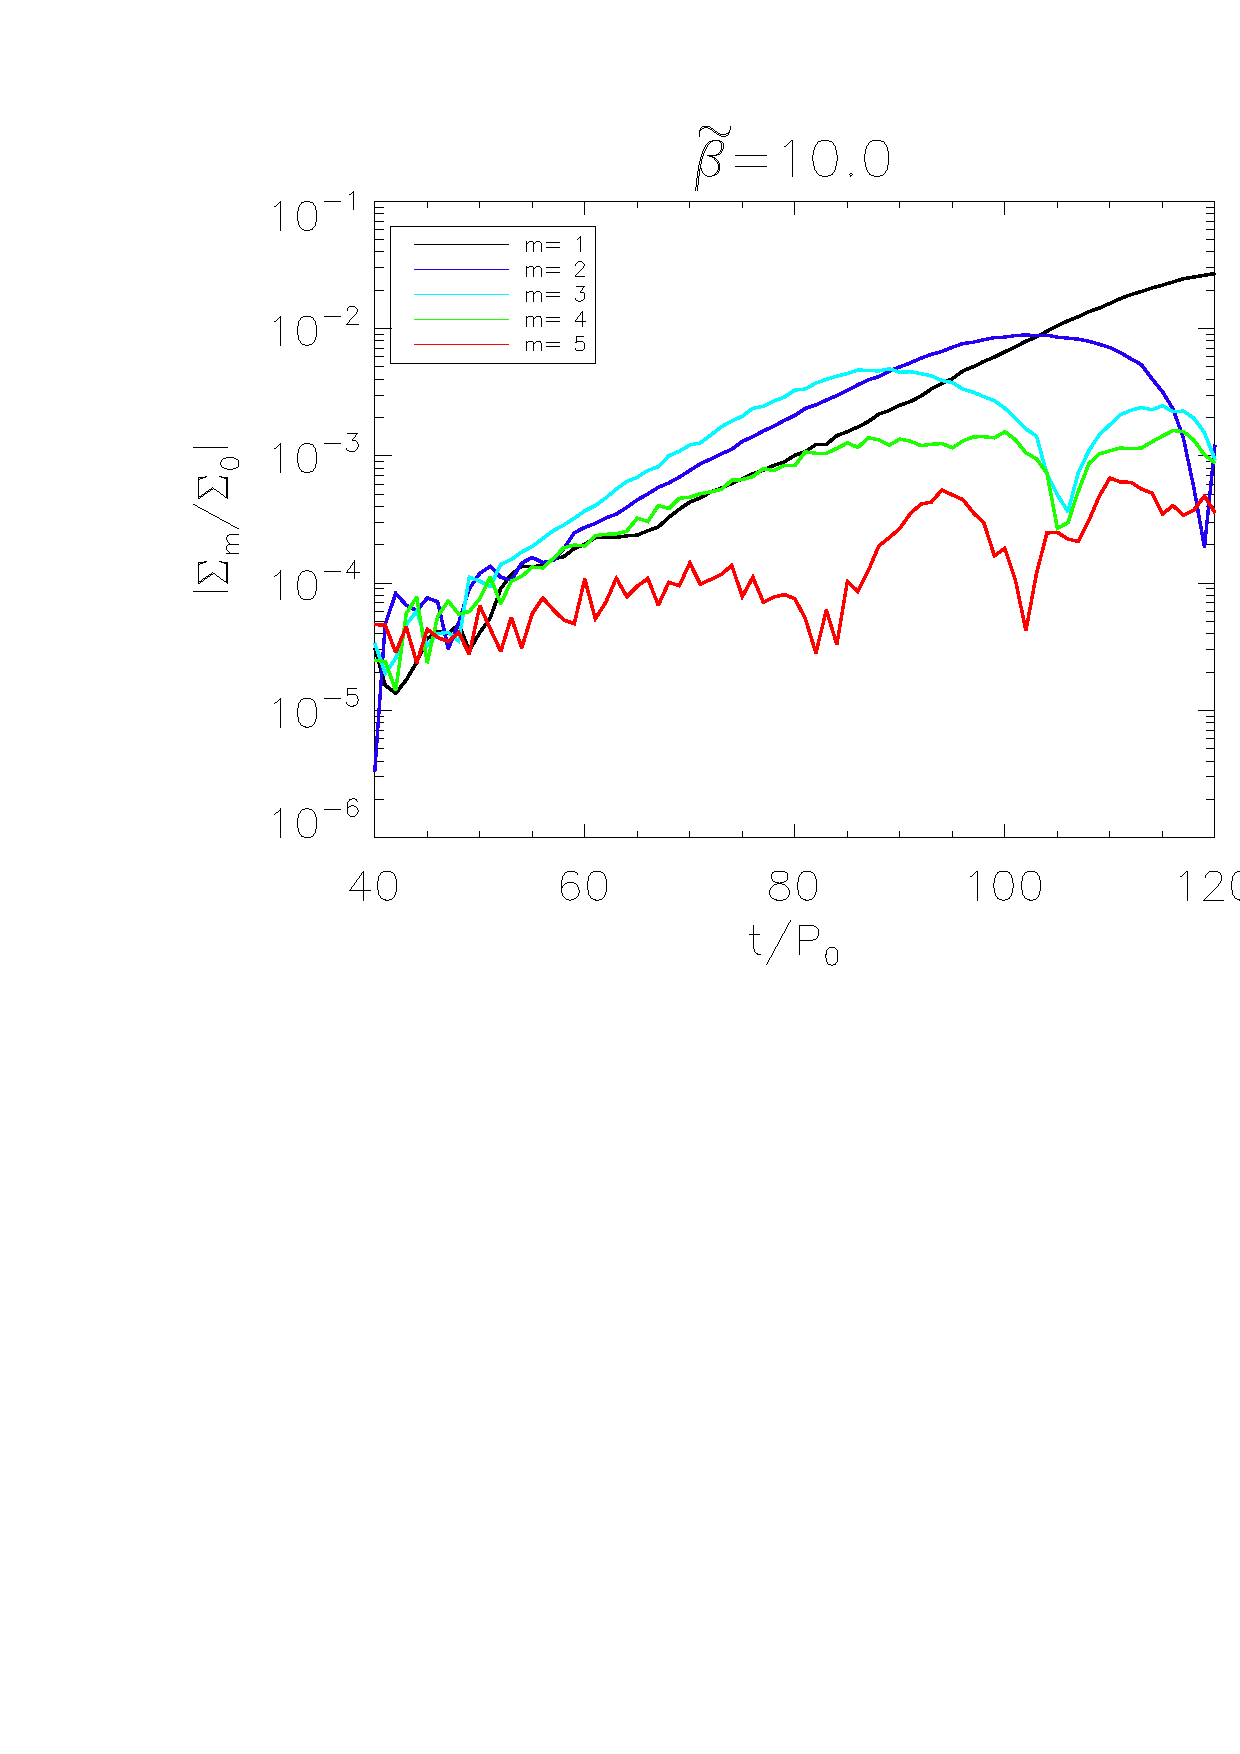
\includegraphics[width=\linewidth,clip=true,trim=1.2cm
    0cm 0cm 0cm]{figures/linear_stability}
  \caption{Evolution of azimuthal Fourier modes of disc surface
    density, non-dimenionlized by the axisymmetric mode for the
    `planet-off' simulations with $\tilde{\beta}=10$. Colours correspond
    to different $m$ values. The $m=3$ component is the fastest growing
    mode during linear growth and has a corresponding
    $\gamma=0.017\Omega(r_p)$. {\bf is the $\Sigma_0$ at
      t=0?} \label{linearmodes}}  
\end{figure}

%%%%%%%%%%%%%%%%%%%%%%%%%%%%%%%%%%%%%%%%%%%%%%%%%%%%%%%%%%%%%%%%%%%%%%%

Table \ref{modetable} show that as
$\tilde{\beta}$ was increased from $ 0.1\rightarrow10$ the dominant
azimuthal Fourier mode decreased from $ m=9\rightarrow3$ and the
respective growth rate decreased from $ \gamma/\Omega(r_p)=0.079
\rightarrow 0.017$. However, despite two orders of magnitude increase in the
cooling time, the instability remains dynamical with growth time
$\lesssim 10P_0$. Snapshots of the instability in $r-\phi$ plane for
the different $\tilde\beta$ are shown in Fig \ref{2Dlinear}. 

These `planet-off' simulations show that gap edges become more stable with
longer cooling times. This is expected because larger $\tilde{\beta}$
result in hotter gap profiles at $t=30P_0$ with less pronounced
generalized vortensity minima. Stabilization with increased
cooling time is therefore due to a smoother basic state for the
instability, as it is more difficult for the planet to open a gap if
the disc is allowed to heat up. 
 

% which result in hotter gaps since the heating
%due
%This is as expected from the
%intial gap profiles, because 
% and the gap forming criteria discussed in the
%previous section. 





\begin{figure*}
  \centering
  \subfigure{
    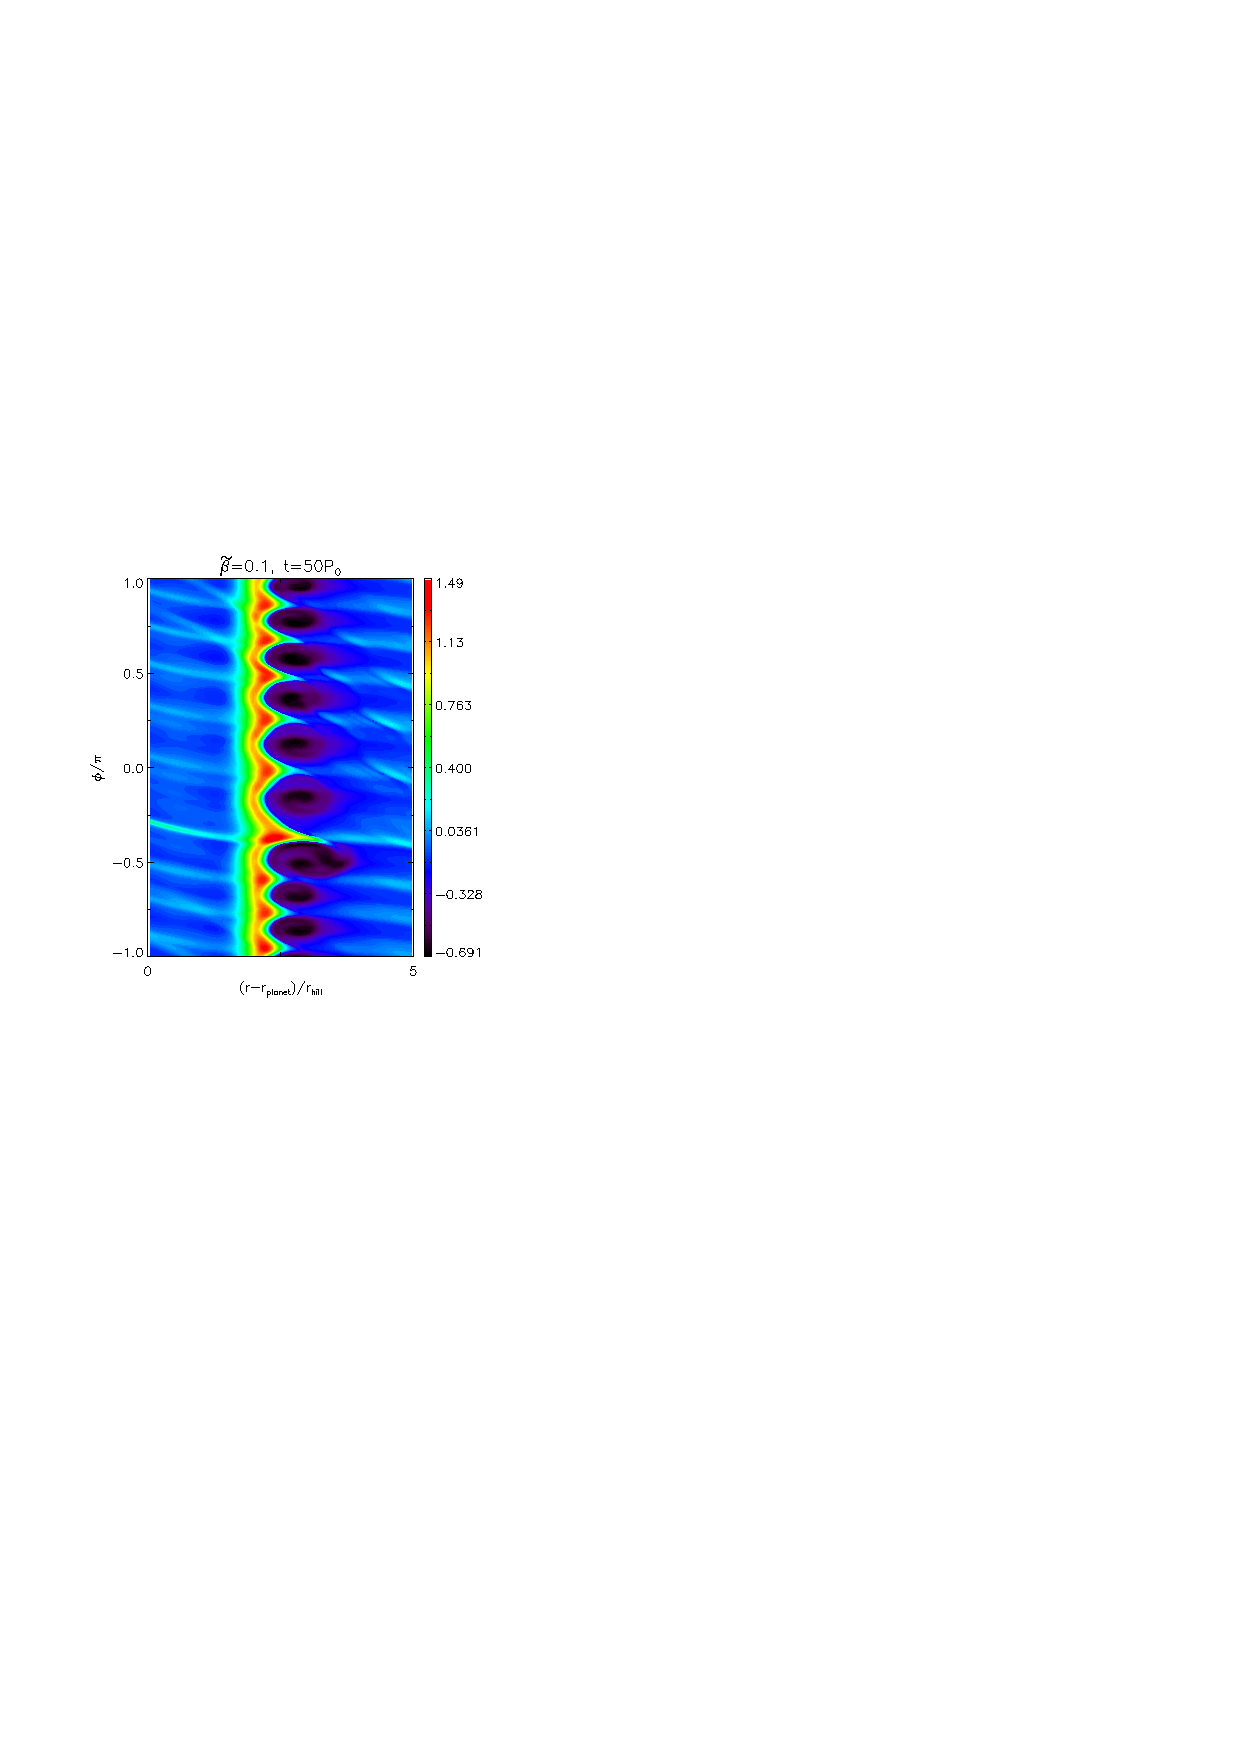
\includegraphics[width=0.3\linewidth]{figures/analysis_gvortensity_lowb}
  }
\hfill
  \subfigure{
    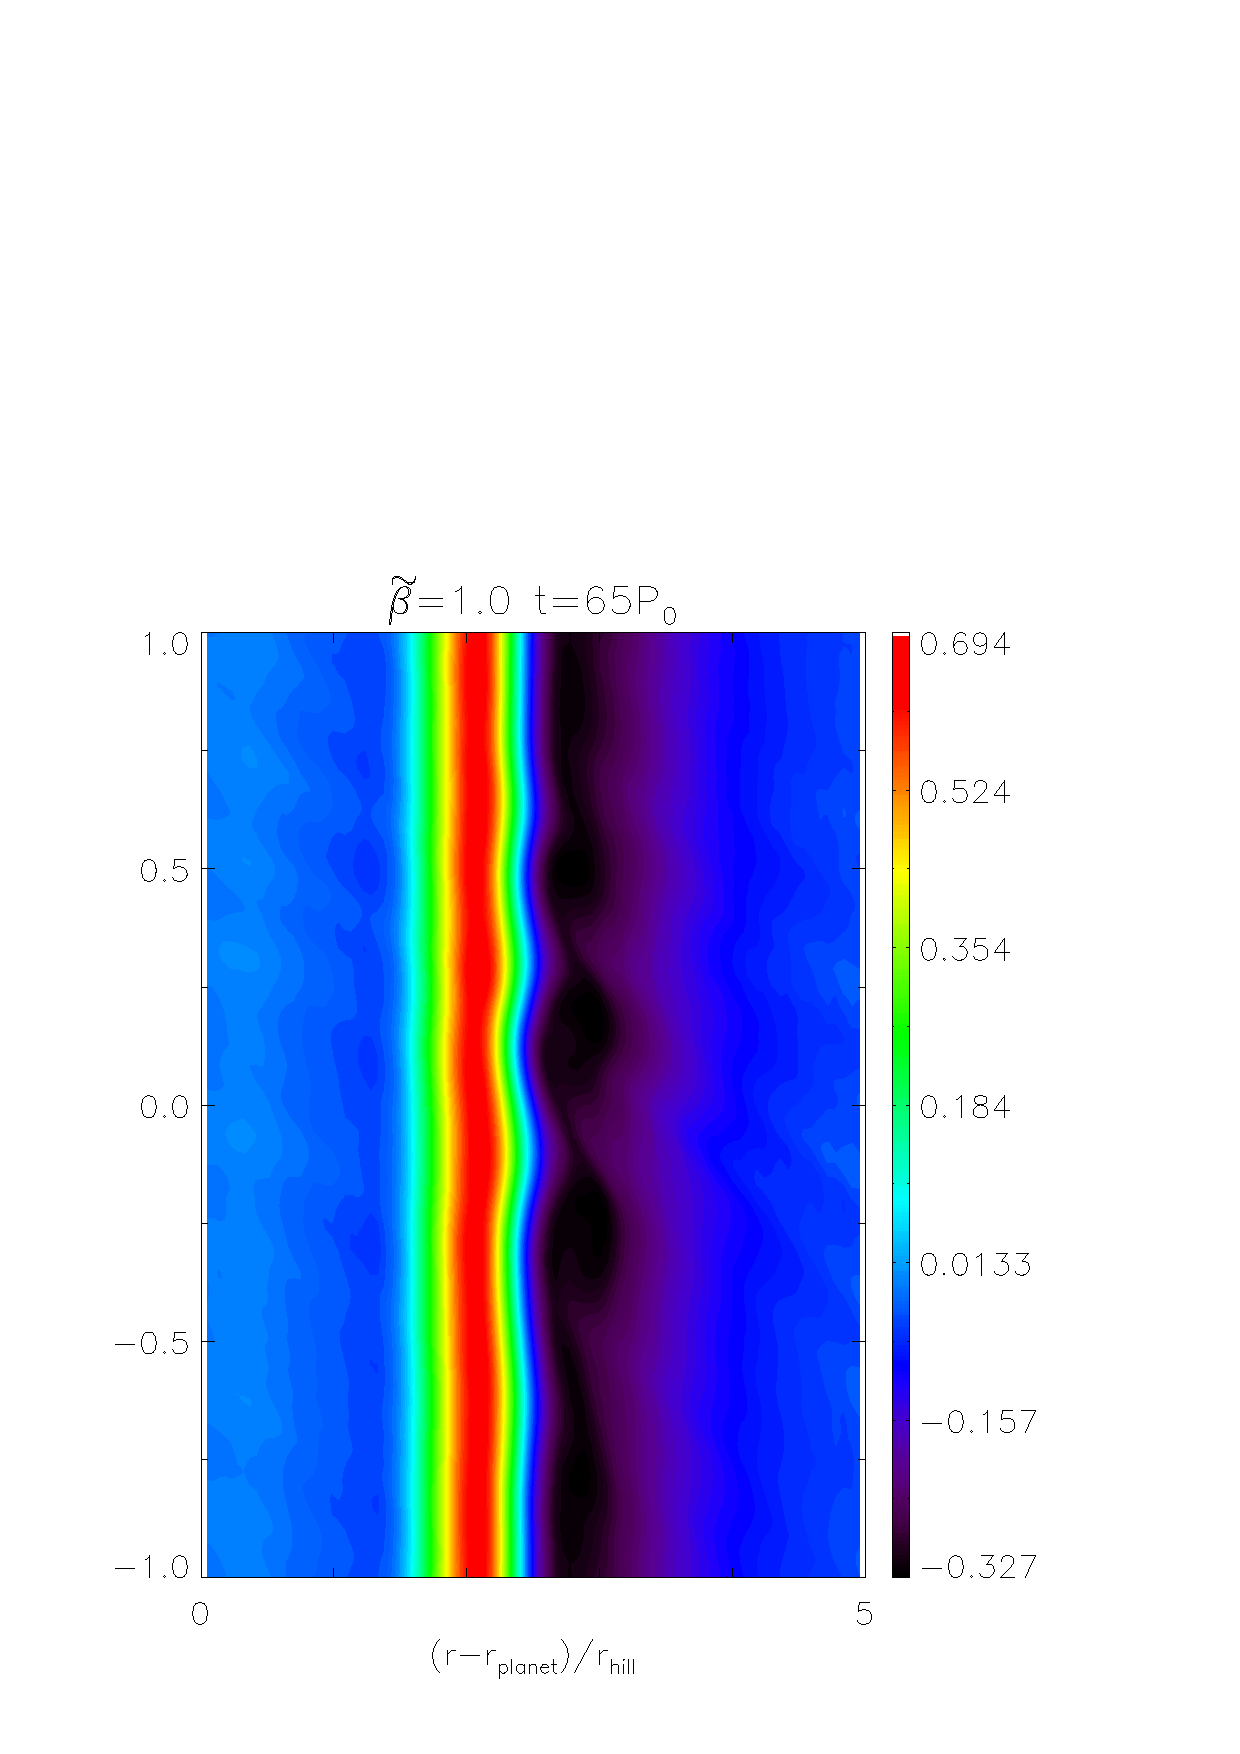
\includegraphics[width=0.3\linewidth]{figures/analysis_gvortensity_medb}
  }
\hfill
  \subfigure{
    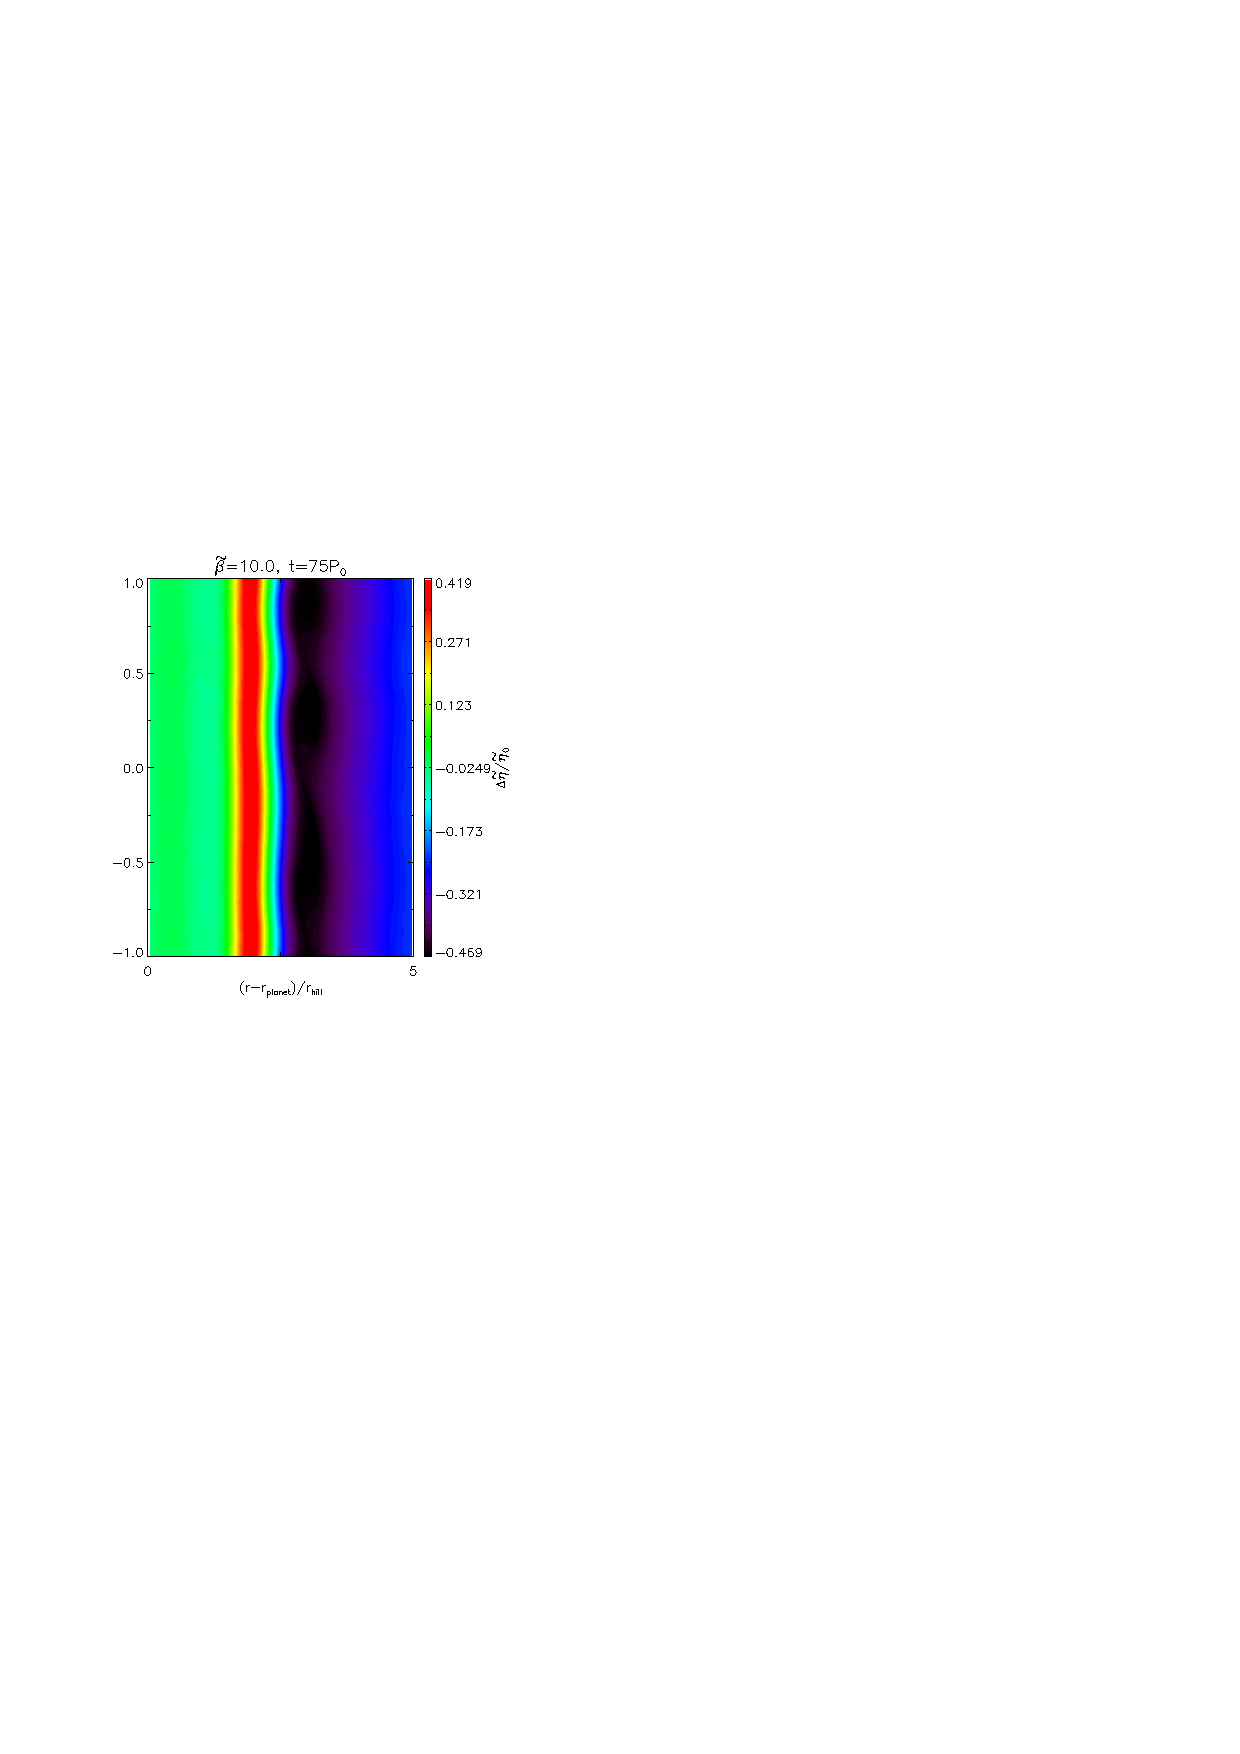
\includegraphics[width=0.3\linewidth]{figures/analysis_gvortensity_highb}
  }  
  \caption{Generalized vortensity perturbation (relative to $t=0$) for
    cases of $\tilde{\beta}=0.1,1,10$ (left,middle,right) during
    the growth of non-axisymmetric modes. The planet potential has
    been switched off.  The number of vortices
    decrease as $\tilde{\beta}$ increases. Note that snapshots are
    taken later because it takes longer for the vortices to grow and
    become visible with increasing cooling time. 
    %    correspondingly increase to capture the longer growth phases of
    %    the instabilities. 
    \label{2Dlinear} {\bf I'm curious to know if plots clearer if
      perturbations are measured relative to t=30? remember t=30 is
      our reference state for instability. But we'll probably keep
      these for consistency (later non-linear plots are all measure
      with respect to t=0).}} 
\end{figure*}

\subsubsection{Nearly adiabatic discs}
\label{adiabatic_section}
%{\bf a case with extrmely long cooling time (or adiabatic run) in
%  order to look at effect of heated gap edge.  prelim result: not
%  important, at t=30, gap edge only heats to $H/r\simeq0.06$ even for
%  purely adiabatic disk. change in $h$ not important for linear
%  perturbations (but important for setting up the basic state). 
%}
The above `planet-off' simulations are not formally linear
stability calculations, because the cooling time is shorter
than the instability growth time, 
%
%as we do not capture the effects of a heated
%disk on the instability growth. 
$t_c<\gamma^{-1}$.  
Thus the disk cools back to its intial value of $h=0.05$
before or during the instability growth, implying we do not have a
steady basic state to formulate a standard linear stability
problem. %This means the disc temperture of $h=0.05$ in the the above cases 

In order to perform a proper linear stability analysis and capture the
effect of a heated gap edge during instability growth, we ran a simulation  with
$\tilde{\beta}=100$, corresponding to an almost adiabtaic disc.  
%To compare our 'planet-off' analysis with a true
%linear stability analysis 
In this simulation the cooling rate is slow enough that the gap 
temperature profile (e.g. middle panel of Fig. \ref{intial1D}) changes
only marginally over the instability growth timescale. %heat is
                                %retained/maintained.   

We find very similar gap profiles and mode growth rates for
$\tilde{\beta}=100$ as with $\tilde{\beta}=10$. The disc heats up to
values $h\simeq0.06$ in the nearly adiabatic case. This is close to
the original temperature of $h=0.05$, so growth rates are not expected
to change significantly according to the linear theory presented in
\citep{li00}. 

According to \cite{li00}, increasing $h$ increases linear growth rates
of the RWI because it is pressure-driven. However, in the case 
of disc-planet interaction, increasing $h$ has a stabilizing effect
through the gap profile because it results in smoother gap
edges. The fact that we observe smaller growth rates as $h$ is
increased indicate that for planetary gaps, the importance of $h$ on
the \emph{linear} RWI is through the setting the gap profile (i.e. basic
state for the instability). 



%results in shallower gaps
%which is expected to be  

%the difference in growth rates between this and the
%original disc temperature of $h=0.05$ changes almost insignificantly
%as shown by linear theory \citep{li00}. 
%Although linear
%theory predicts higher growth rates with increasing $h$ 

%This indicate that a
%continuously hot gap edge is not as important for development of
%vortices as the heating effects on the formation of the intial gap
%state. 


{\bf
If there's time, repeat planet off simulations but keep the planet on
until $t=40P_0$ or $50P_0$. Look at stability properties when the gaps
are generally deeper (including the nearly adiabatic case). Although
with the planet instability may already appear by $t=40P_0$, the
azimtuhal average performed prior to perturbations will erase it. 
}


%%%%%%%%%%%%%%%%%%%%%%%%%%%%%%%%%%%%%%%%%%%%%%%%%%%%%%%%%%%%%%%%%%%%%

\section{Non-linear evolution of
  gap-edge vortices with finite cooling time} 
%{\bf main fig: vortex amplitude v.s. time for diff beta. enough data
%  to plot vortex lifetime v.s. beta? table: 
%  averaged quantities over quasi-steady state: aspect-ratio (to
%  compare with fu at al), rossby number (vortex strength
%  v.s. cooling?), maybe alpha visc. vortex size: visible difference?  
%  only inviscid cases. describe evolution of one case. main
%  conclusion: longer vortex lifetime with increasing cooling time (up
%  to some optimal timescale). vortex death: induced-shock and/or
%  smoothing the gap edge. describe simulation setup, resolution?
%  should mention that results consistent with lower-resolution prelim
%  runs. maybe torques? 
%}

Long term simulation of edge vortices were done for
$\tilde{\beta}=0.1,0.5,1.0,5.0,10.0$ up to a total of
$2000P_0$. Planets were left free to interact dynamiclly with the disk
and vortices after $t=30P_0$ as apposed to previous section. These
simulations were less resolved with $(N_r,N_{\phi})=(512,1024)$ in
order for them to be computationally economical. An open boundry
condition was used in the outer edge of
$r_{\mathrm{out}}=45r_{\mathrm{in}}$ allowing significant room for
linblad resonances of the vortices. 

After the semi-linear growth of vortices, vortex merger effects take
hold and by $150P_0$ for all $\tilde\beta$ values, only $m=1$ vortex
modes exist. Plots of the amplitude of the $m=1$ mode for the
different $\tilde\beta$ cases are shown in
Fig~\ref{lifetimeplot}. These instabilities stay in quasi-steady
states for $>1000P_0$ in most cases, in which they grow in intensity
and reaching overdenisities almost 10 times the intial local
density. The growth of these vortices are supplied by the continuous
generation of vorticity by the planet-disk interactions. Eventually
the $m=1$ amplitudes are also characterized by sudden large drops of
vortex intensity which happen over timescales of $50P_0$. After these
drops the instability is never seen to reform at such large over
densities and density bumps are never larger than the planet induced
shocks. We designate the time of these amplitude drops as the lifetime
of the quasi-steady vortex.  

Rossby values have dynamics that are coupled with the lifetime and
$m=1$ amplitude of the vortices. As the vortex forms it has a
charcteristic value of $Ro\approx-0.1$ indicating anti-cyclonic
motion. As the $m=1$ amplitude grows the relative spin of the vortex
continuously grows along with it, reaching values of
$Ro\approx-0.4$. As the vortex dies off as described above the
associated Rossby number of the vortex accordingly quickly approaches
0. 

The sudden dissipation of these vortices seem to be a result of the
vortices shocking the system. Measurements of the Mach number near the
vortices show large increases in value when the vortex is dissipating
which indicates that the system is more susceptible to shocks. Also
gradients of surface density are seen to spike up in wake like
features around the vortex during dissipation which is also indicative
of shocks. Of note is also that the large overdensity the vortex
creates during it's quasi-steady state distorts the background
disk. So as the vortex grows in intensity it alters the intial gap
structure that formulated its growth. 

Contradictory to our `planet-off' simulations, vortex lifetimes did
not monotonicly depend on intial edge stability and from our
simulations we find that there is $t_{\mathrm{coo}l}$ which optimizes
the vortex lifetime as seen in Fig~\ref{lifetimeplot}. Increasing
$\tilde\beta$ correspondingly increased the lifetime of the vortex up
to a critical value for $\tilde{\beta}=5.0$ which had a lifetime that
lasted beyond the simulation time of $2000P_0$. Cooling rates with
$\tilde\beta>5.0$ showed lifetimes that were well below the max
lifetime. By analyzing the aspect ratio of the corotation region
around the vortex we find that longest lifetime $\tilde\beta=5.0$ disk
corresponds to $h\approx0.06$ which is a result similarily found by
\citet{fu14} to be the optimum lifetime for long-term simulations of
isothermal disks with varying intial temperature profiles $h$. 

Competing effects of gap stability with $t_{\mathrm{coo}l}$ result in
the the non-montonic form of the lifetime. As the $\tilde\beta$
increases so does the stability of the gap edge as seen in
section~\ref{linear}, however as $\tilde\beta$ increases so does the
$c_{\mathrm{iso}}$ which is known from theory to effect the growth of
instability \citep{li00}. Thus increasing $\tilde\beta$ increases the
sound speed $c_{\mathrm{iso}}$ and likewise the gap instability up to
a certain point in which the effects of the more stable gap edge
becomes a significant effect. The correlation of growth rate and sound
speed is non-negligible as in previous `planet-off' case as the disk
now can reach values of $h\simeq0.08$ for very slow cooling and the
importance of the effect can be imagined to accumulate over the now
considerably longer timescale. These effects dictate when then the
vortex reaches the critical value in which it shocks the system that
subsequently causes disspation and hence the lifetime fo the vortex. 

\begin{figure}
  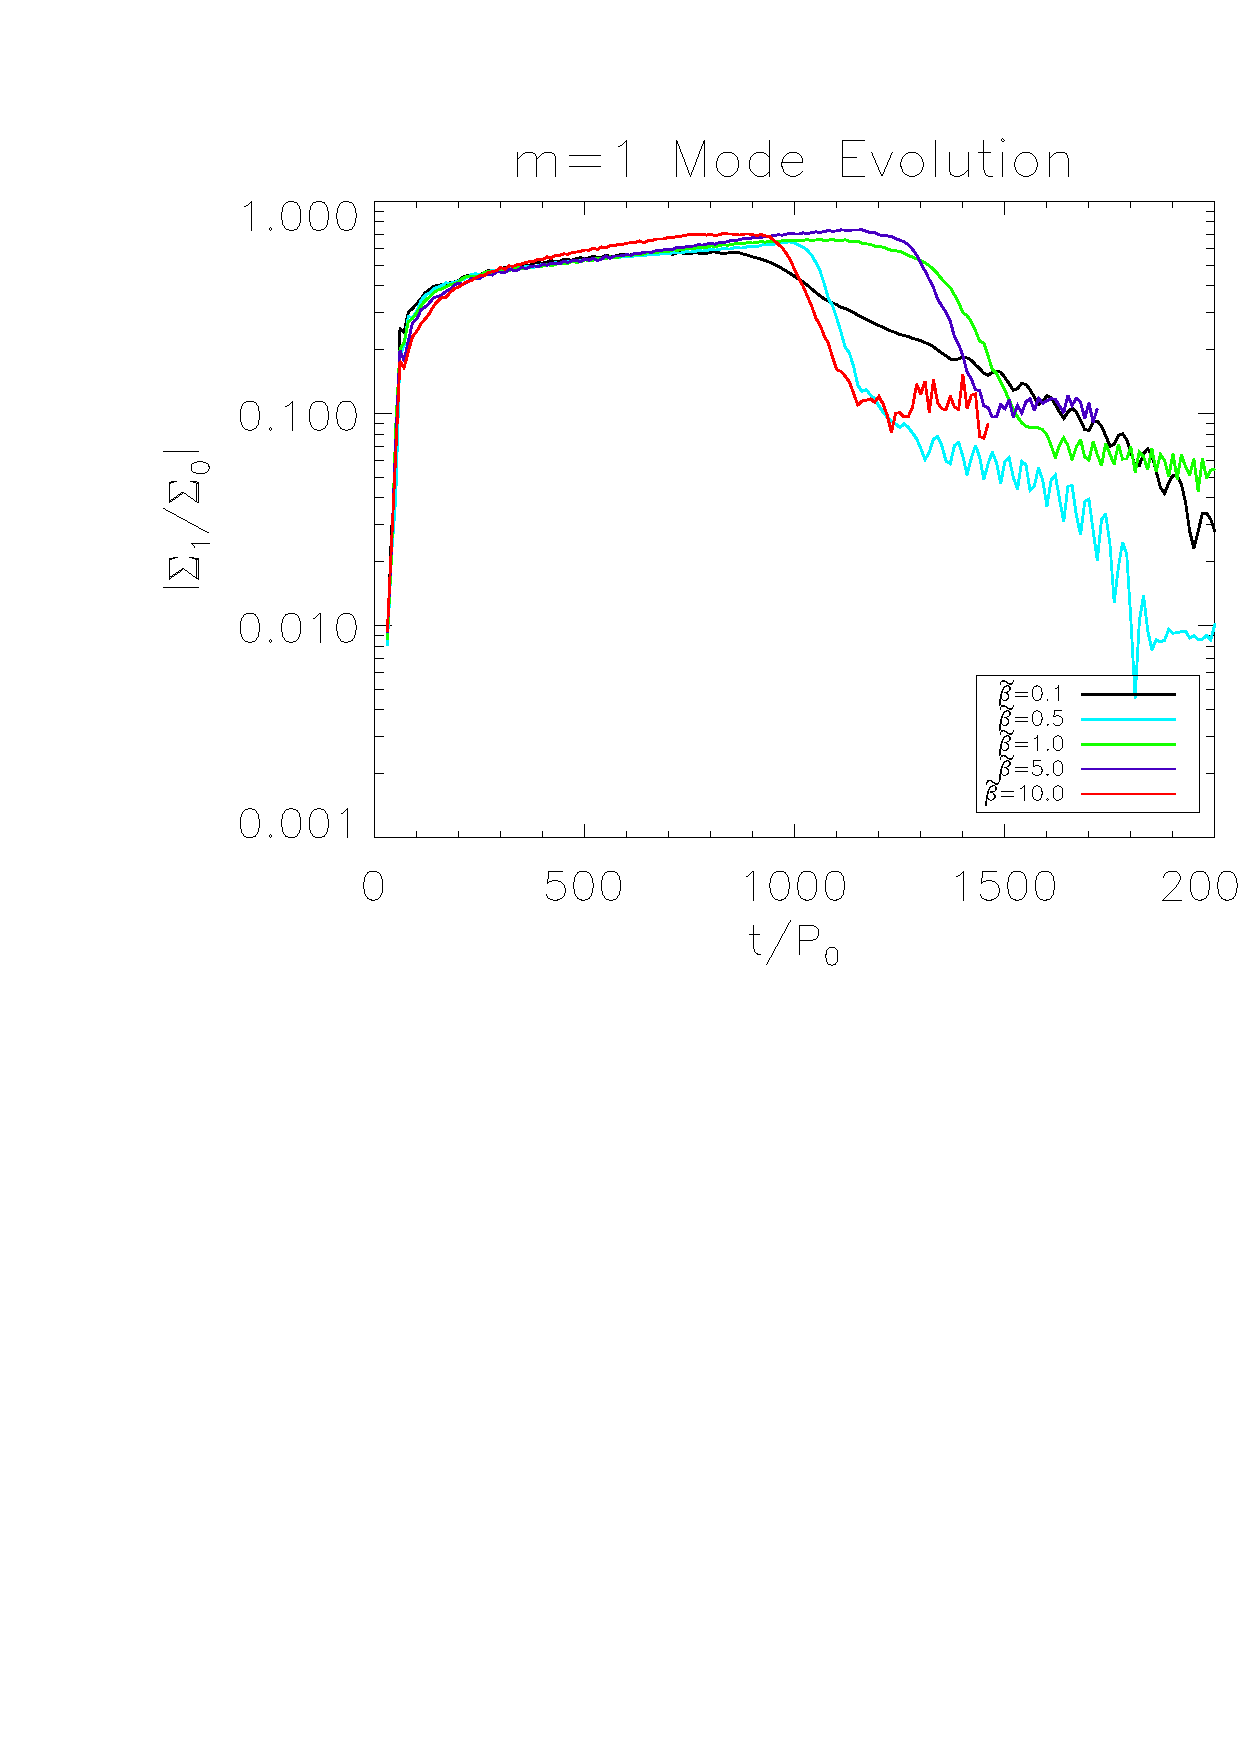
\includegraphics[width=\linewidth,clip=true,trim=0.5cm
    0cm 0cm 1cm]{figures/longterm_stability}
  \caption{Log plot of the $m=1$ mode non-dimenionlized by the $m=0$
    background mode for longterm non-linear simulations corrsponding
    to vortex lifetime. The longest living mode correpsonds to
    $\tilde\beta=5.0$ (the red line). \label{lifetimeplot}} 
\end{figure}

\begin{figure}
  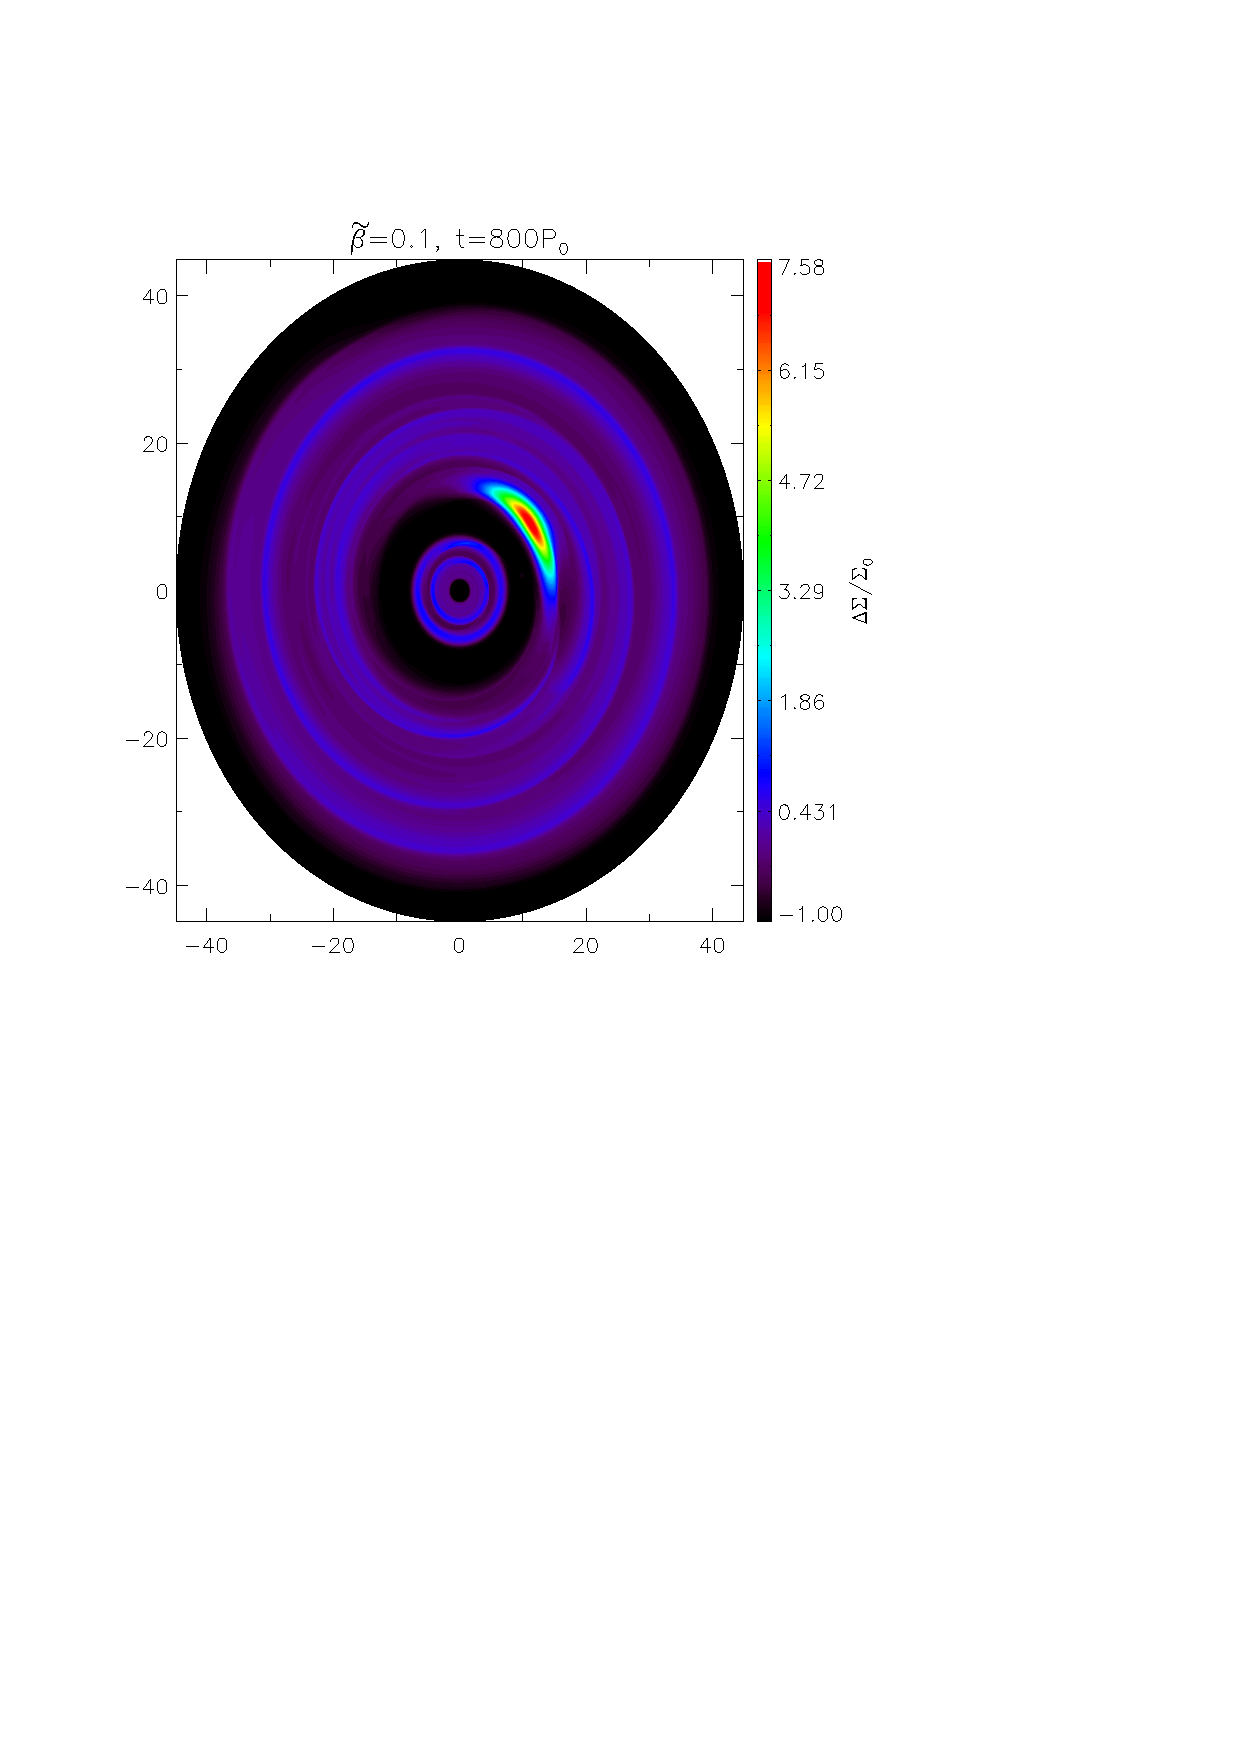
\includegraphics[width=\linewidth,height=\linewidth]{figures/vortex2D}
  \caption{Cartesian plot of relative density pertibation for
    $\tilde\beta=0.1$ vortex case during the quasi-steady state. The
    large scale non-axisyemetric $m=1$ overdensity can be
    seen. \label{Vortex2D}} 
\end{figure}

%\begin{figure}
%   \includegraphics[scale=.42]{figures/stability_vis6betalow.ps}
%   \caption{Same as Fig. \ref{stability_vis9lowb} but $\hat{\nu}=10^{-6}$ and $\tilde{\beta}=0.1$. }
% \label{stability_vis6lowb)}
% \end{figure}

%\begin{figure}
%   \includegraphics[scale=.42]{figures/stability_vis6betamed.ps}
%   \caption{Same as Fig. \ref{stability_vis9lowb} but $\hat{\nu}=10^{-6}$ and $\tilde{\beta}=1.0$. }
% \label{stability_vis6medb)}
% \end{figure}
%Same as \ref{stability_vis9lowb} but $\hat{\nu}=10^{-6}$ and $\tilde{\beta}=1.0$. 


%we checked that open bc doesn't affect gap structure
%checked that t=200 plots are similar to t=100 

%surface density plot

%aspect-ratio plot

%general vortensity plot 



%% \begin{figure}
%%   \includegraphics[scale=.42,clip=true,trim=0cm 1.8cm 0cm 0cm]{figures/compare_profiles_dens020.ps}\\
%%   \includegraphics[scale=.42]{figures/compare_profiles_h020.ps}
%%   \caption{Steady-state gap profiles in a low mass viscous disc. The
%%     surface density perturbation (top) and disc aspect-ratio (bottom)
%%     are shown as a function of the cooling parameter:  
%%     $\tbeta=0.1$ (solid, fast cooling), $\tbeta=1$ (dotted,
%%     moderate cooling) and $\tbeta=10$ (dashed, slow
%%     cooling). \label{lvisc_steady_gap}}  
%% \end{figure}



%% \begin{figure}
%%   \includegraphics[scale=.42]{figures/compare_profiles_gvort020.ps}
%%   \caption{Gap structure in a low mass viscous disc, in terms of the
%%     perturbed generalized vortensity as a function of the cooling
%%     parameter. \label{lvisc_steady_gvort}} 
%% \end{figure}


%%\section{Gaps in massive discs (MKL)}
%% We first examine disc models with $Q_o=1.5$. We set the physical
%% viscosity $\hat{\nu}=10^{-9}$, so that the only energy source is
%% through shock-heating (via artificial viscosity) and the $\mathcal{C}$
%% function when $e\Sigma<e_i\Sigma_i$. The numerical resolution is
%% $N_r\times N_\phi = 512\times 1024$.   

%% %Since we are primarily concerened with gap stability, it is important
%% %to first examine the gap structured opened by the planet as a function
%% %of cooling. 
%% Fig. \ref{gvort1d_q1d5} compares the gap structure in terms of the GV profile for three
%% levels of cooling: $\tilde{\beta}=0.1$, $\tilde{\beta}=1$ and
%% $\tbeta=10$. For convenience we will refer to these cases as fast,
%% intermediate and slow cooling, respectively. The snapshot is taken at
%% $t=30P_0$, just after the planet is fully introduced. 

%% In terms of the GV profile, the qualitative features of the planetary
%% gap --- localized GV extrema at the gap edges --- remain unchanged
%% despite two orders of magnitude difference in the cooling rate.   


%% \begin{figure}
%% %  \includegraphics[scale=.42,clip=true,trim=0cm 1.8cm 0cm 0cm]{figures/dens1d_q1d5_003_global.ps}\\
%% %  \includegraphics[scale=.42]{figures/gvort1d_q1d5_003_global.ps}
%%   \caption{Gap structure in terms of the perturbed surface density
%%     (top) and perturbed generalized
%%     vortensity (bottom), as a function of the cooling parameter:  
%%     $\tbeta=0.1$ (solid, fast cooling), $\tbeta=1$ (dotted,
%%     intermediate cooling) and $\tbeta=10$ (dashed, slow
%%     cooling). \label{gvort1d_q1d5}} 
%% \end{figure}

%% \begin{figure*}
%% %  \includegraphics[scale=.55,clip=true,trim=0cm 0cm 0cm
%% %    0cm]{figures/noniso0_HR_dens004}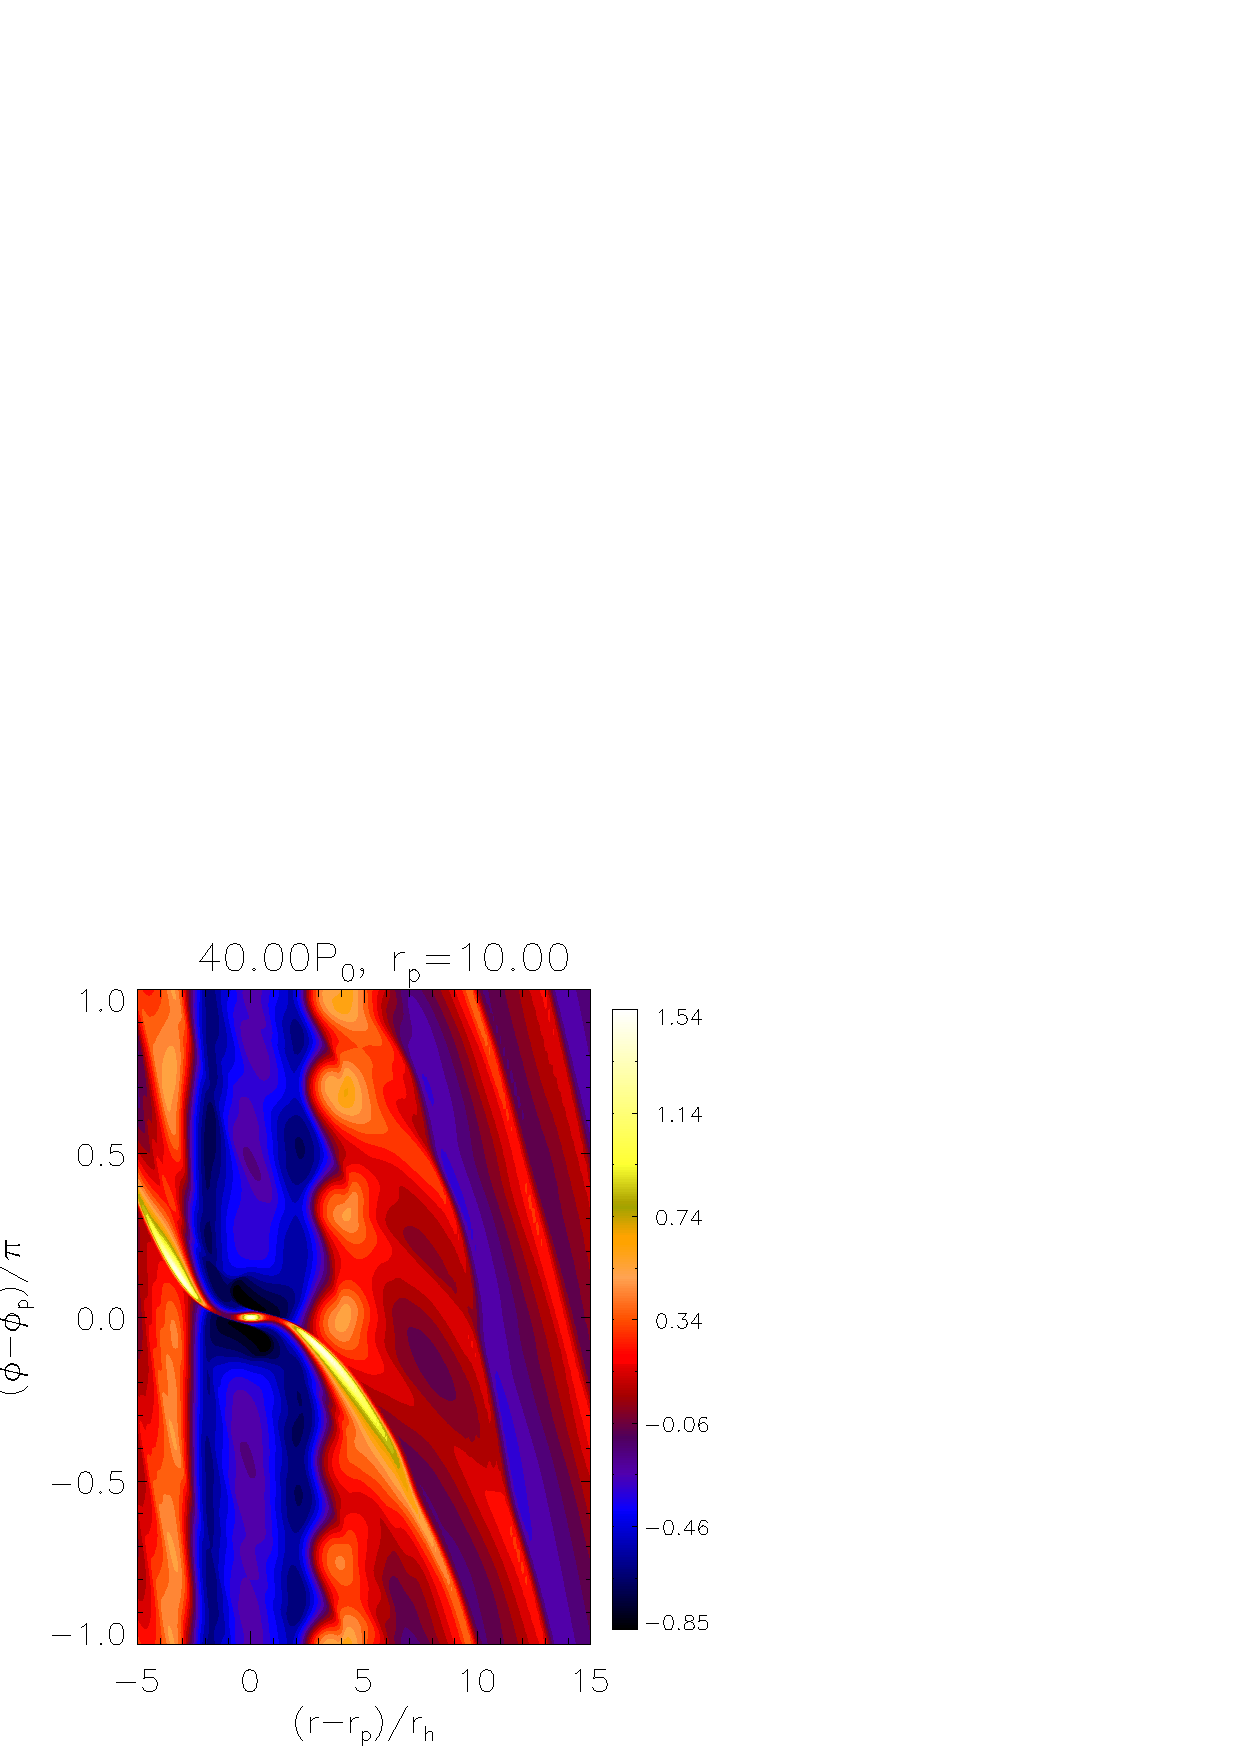
\includegraphics[scale=.55,clip=true,trim=2.26cm 0cm 0cm
%% %    0cm]{figures/noniso1_HR_dens004}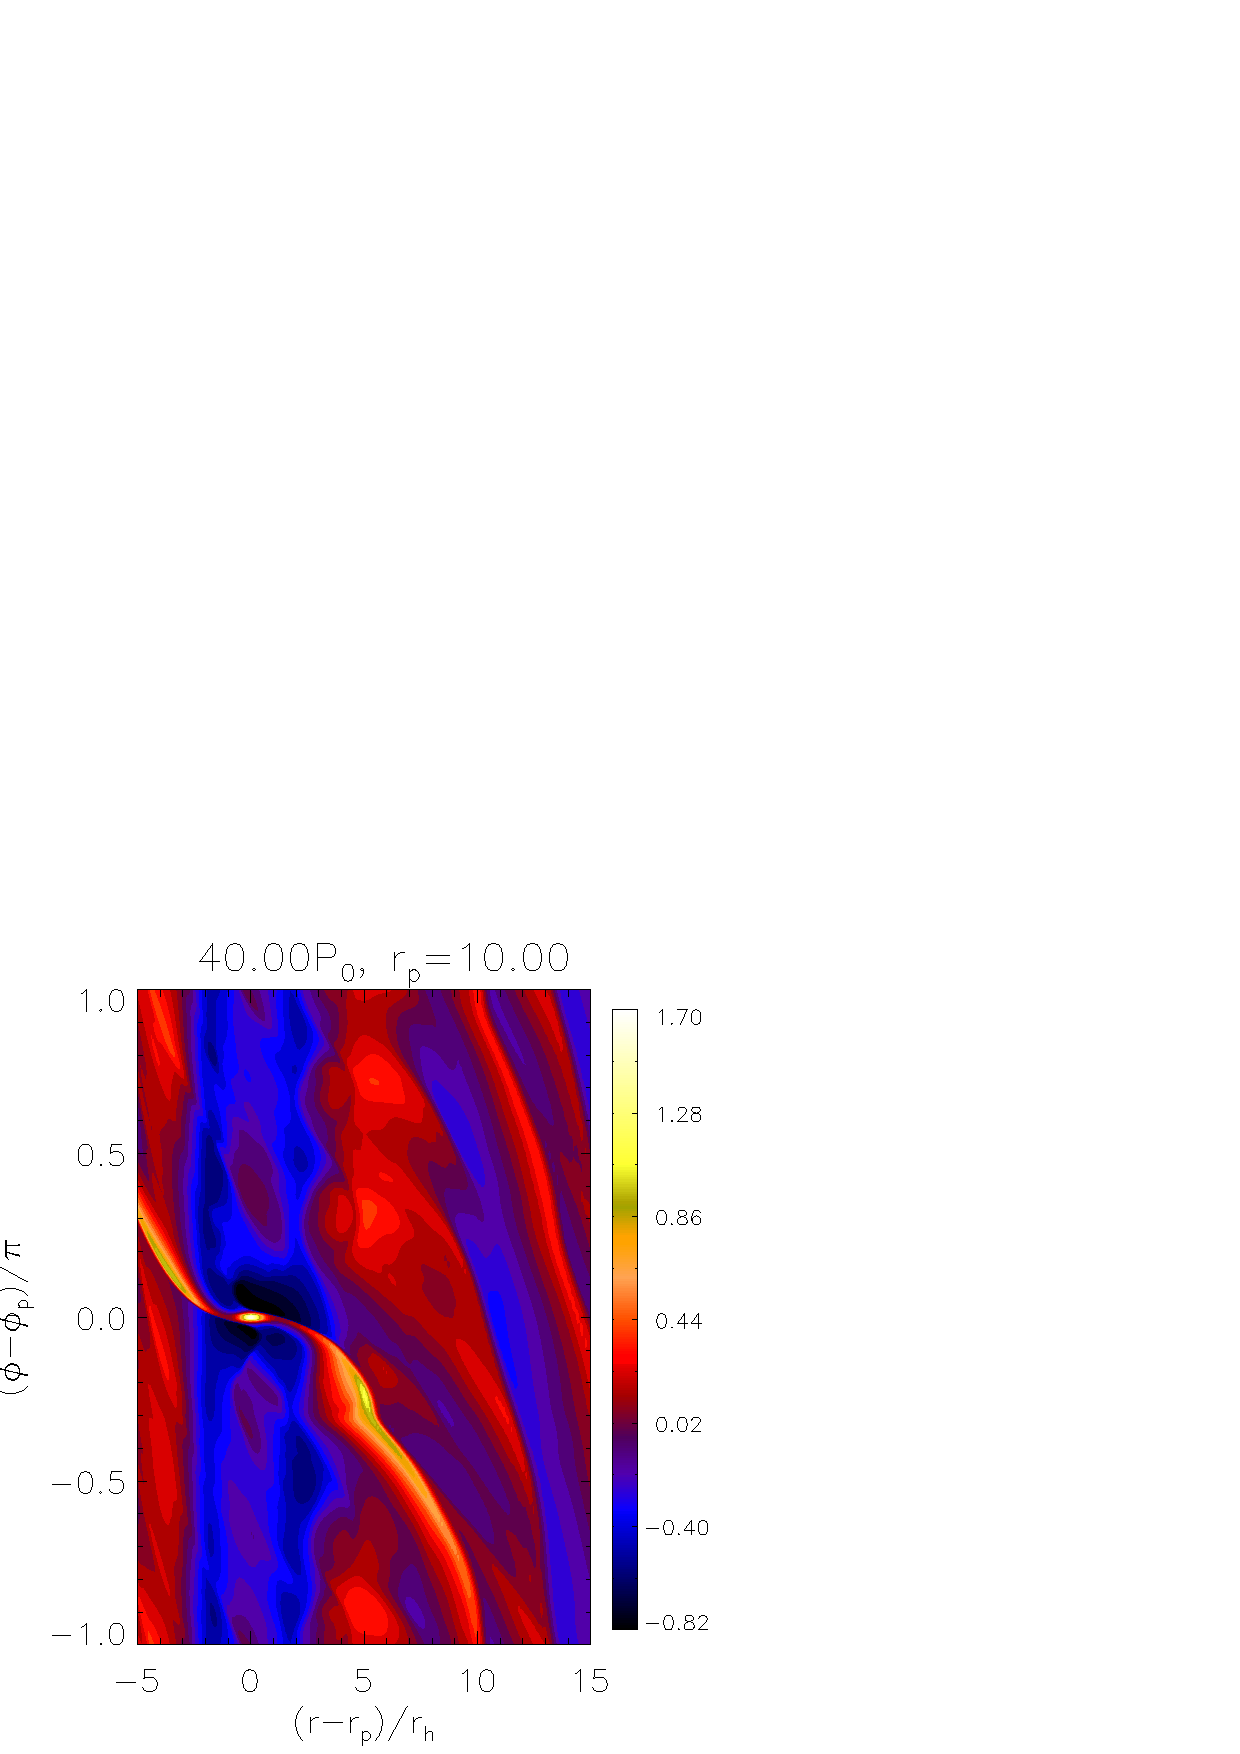
\includegraphics[scale=.55,clip=true,trim=2.26cm 0cm 0cm
%% %    0cm]{figures/noniso2_HR_dens004}
%%   \caption{Gap instability in the heavy disc model, as a function of
%%     the cooling parameter: $\tbeta=0.1$ (left), $\tbeta=1$ (middle)
%%     and $\tbeta=10$ (right). The relative surface density
%%     perturbation is shown. \label{polarxy_q1d5}} 
%% \end{figure*}
